%势阱
\begin{introduction}
    \item 无限深势阱
    \item 有限深势阱与半无限深势阱
    \item 深势阱的应用
    \item 自由粒子的散射问题
\end{introduction}
本节我们的目标是求解势能函数为常数或是无穷大时的态与能量本征值。这些模型虽然粗糙,但是已经能够对一些深刻的物理概念作出近似了。下面我们一一讨论:
\footnote{在本章中,如果没有说明,则只考虑一维情况。}
\section{无限深势阱}
我们考虑以下势场(见图\ref{fig3:inftypotential}):
\begin{align}
V(x)=\left\{
    \begin{array}{ll}
       0  &  0\leq x\leq a\\
       \infty  & elsewhere 
    \end{array}
\right.
\end{align}

\begin{figure}[htp]
    \centering
    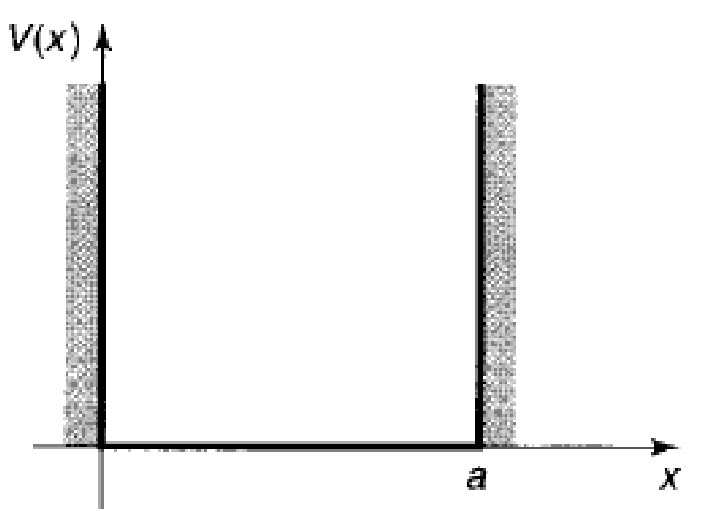
\includegraphics[width=0.5\textwidth]{figure/inftypotential.jpg}
    \caption{无限深势阱的势能示意图}
    \label{fig3:inftypotential}
\end{figure}

由于势场在除了$0\leq x\leq a$处都是无穷大的,因此粒子被束缚在了[0,a]中,我们只需要讨论这个范围中的运动情况即可。此时的Schrodinger方程为:
\begin{equation}
    E\psi =-\frac{\hbar^2}{2m}\frac{d^2\psi}{dx^2}
\end{equation}

其中E是能量本征态,我们可以将上式简写为:
\begin{equation}\label{equ3:string}
\frac{d^2\psi}{dx^2}+k^2\psi =0    
\end{equation}

其中$k=\sqrt{\frac{2mE}{\hbar^2}}$,求解微分方程得到该方程的通解:
\begin{equation}
    \psi =Acoskx+Bsinkx
\end{equation}

随后我们考虑初值问题,由于波函数一定是单值,连续,归一的,而边界上,波函数的势能无限大,因此出现粒子的概率一定为0,即波函数在边界上的取值为0:
\begin{equation}
    \psi(0)=\psi(a)=0
\end{equation}

当$x=0$,我们得到$A=0$;进一步的,当$x=a$,我们得到$Bsinka=0$。由于我们需要一个有意义的波函数,因此在这里$B\ne 0$(否则波函数恒为0)。于是我们可以得到边界条件为:$sinka=0$,即
\begin{equation}
    ka=n\pi ,n=0,\pm 1,\pm 2,\ldots
\end{equation}

根据边界条件,我们可以知道能量本征值的关系:
\begin{equation}
    E=\frac{k^2\hbar}{2m}=\frac{n^2\pi^2 \hbar^2}{2a^2m},n=0,1,2,\ldots 
\end{equation}

由于当$n<0$时,能量本征值与$n>0$时一一对应,并不产生新的结果。因此我们可以人为定义n的取值为正整数。最后我们通过归一化求出归一化因子B:
\begin{equation}
    \int_0^a |B|^2sin^2kx dx =1 \Rightarrow B=\sqrt{\frac{2}{a}}
\end{equation}

于是我们求得了最终的本征函数$\psi_n(x)$:
\begin{equation}
    \psi_n(x)=\sqrt{\frac{2}{a}}sin(\frac{n\pi}{a}x)
\end{equation}

对于这个简单模型,还可以从波动的角度理解:由式\ref{equ3:string},我们可以知道此时定态Schrodinger方程是一个弦振动方程。更进一步,考虑到边界条件,这应该是一个两端固定的弦振动方程,因此我们可以将这个方程的解看作一种驻波,此时势阱宽a满足驻波条件:
\begin{equation}
    a=\frac{\lambda}{2}\cdot n
\end{equation}

这里的$\lambda$是De Brogile 驻波对应的波长。

\begin{figure}[htp]
    \centering
    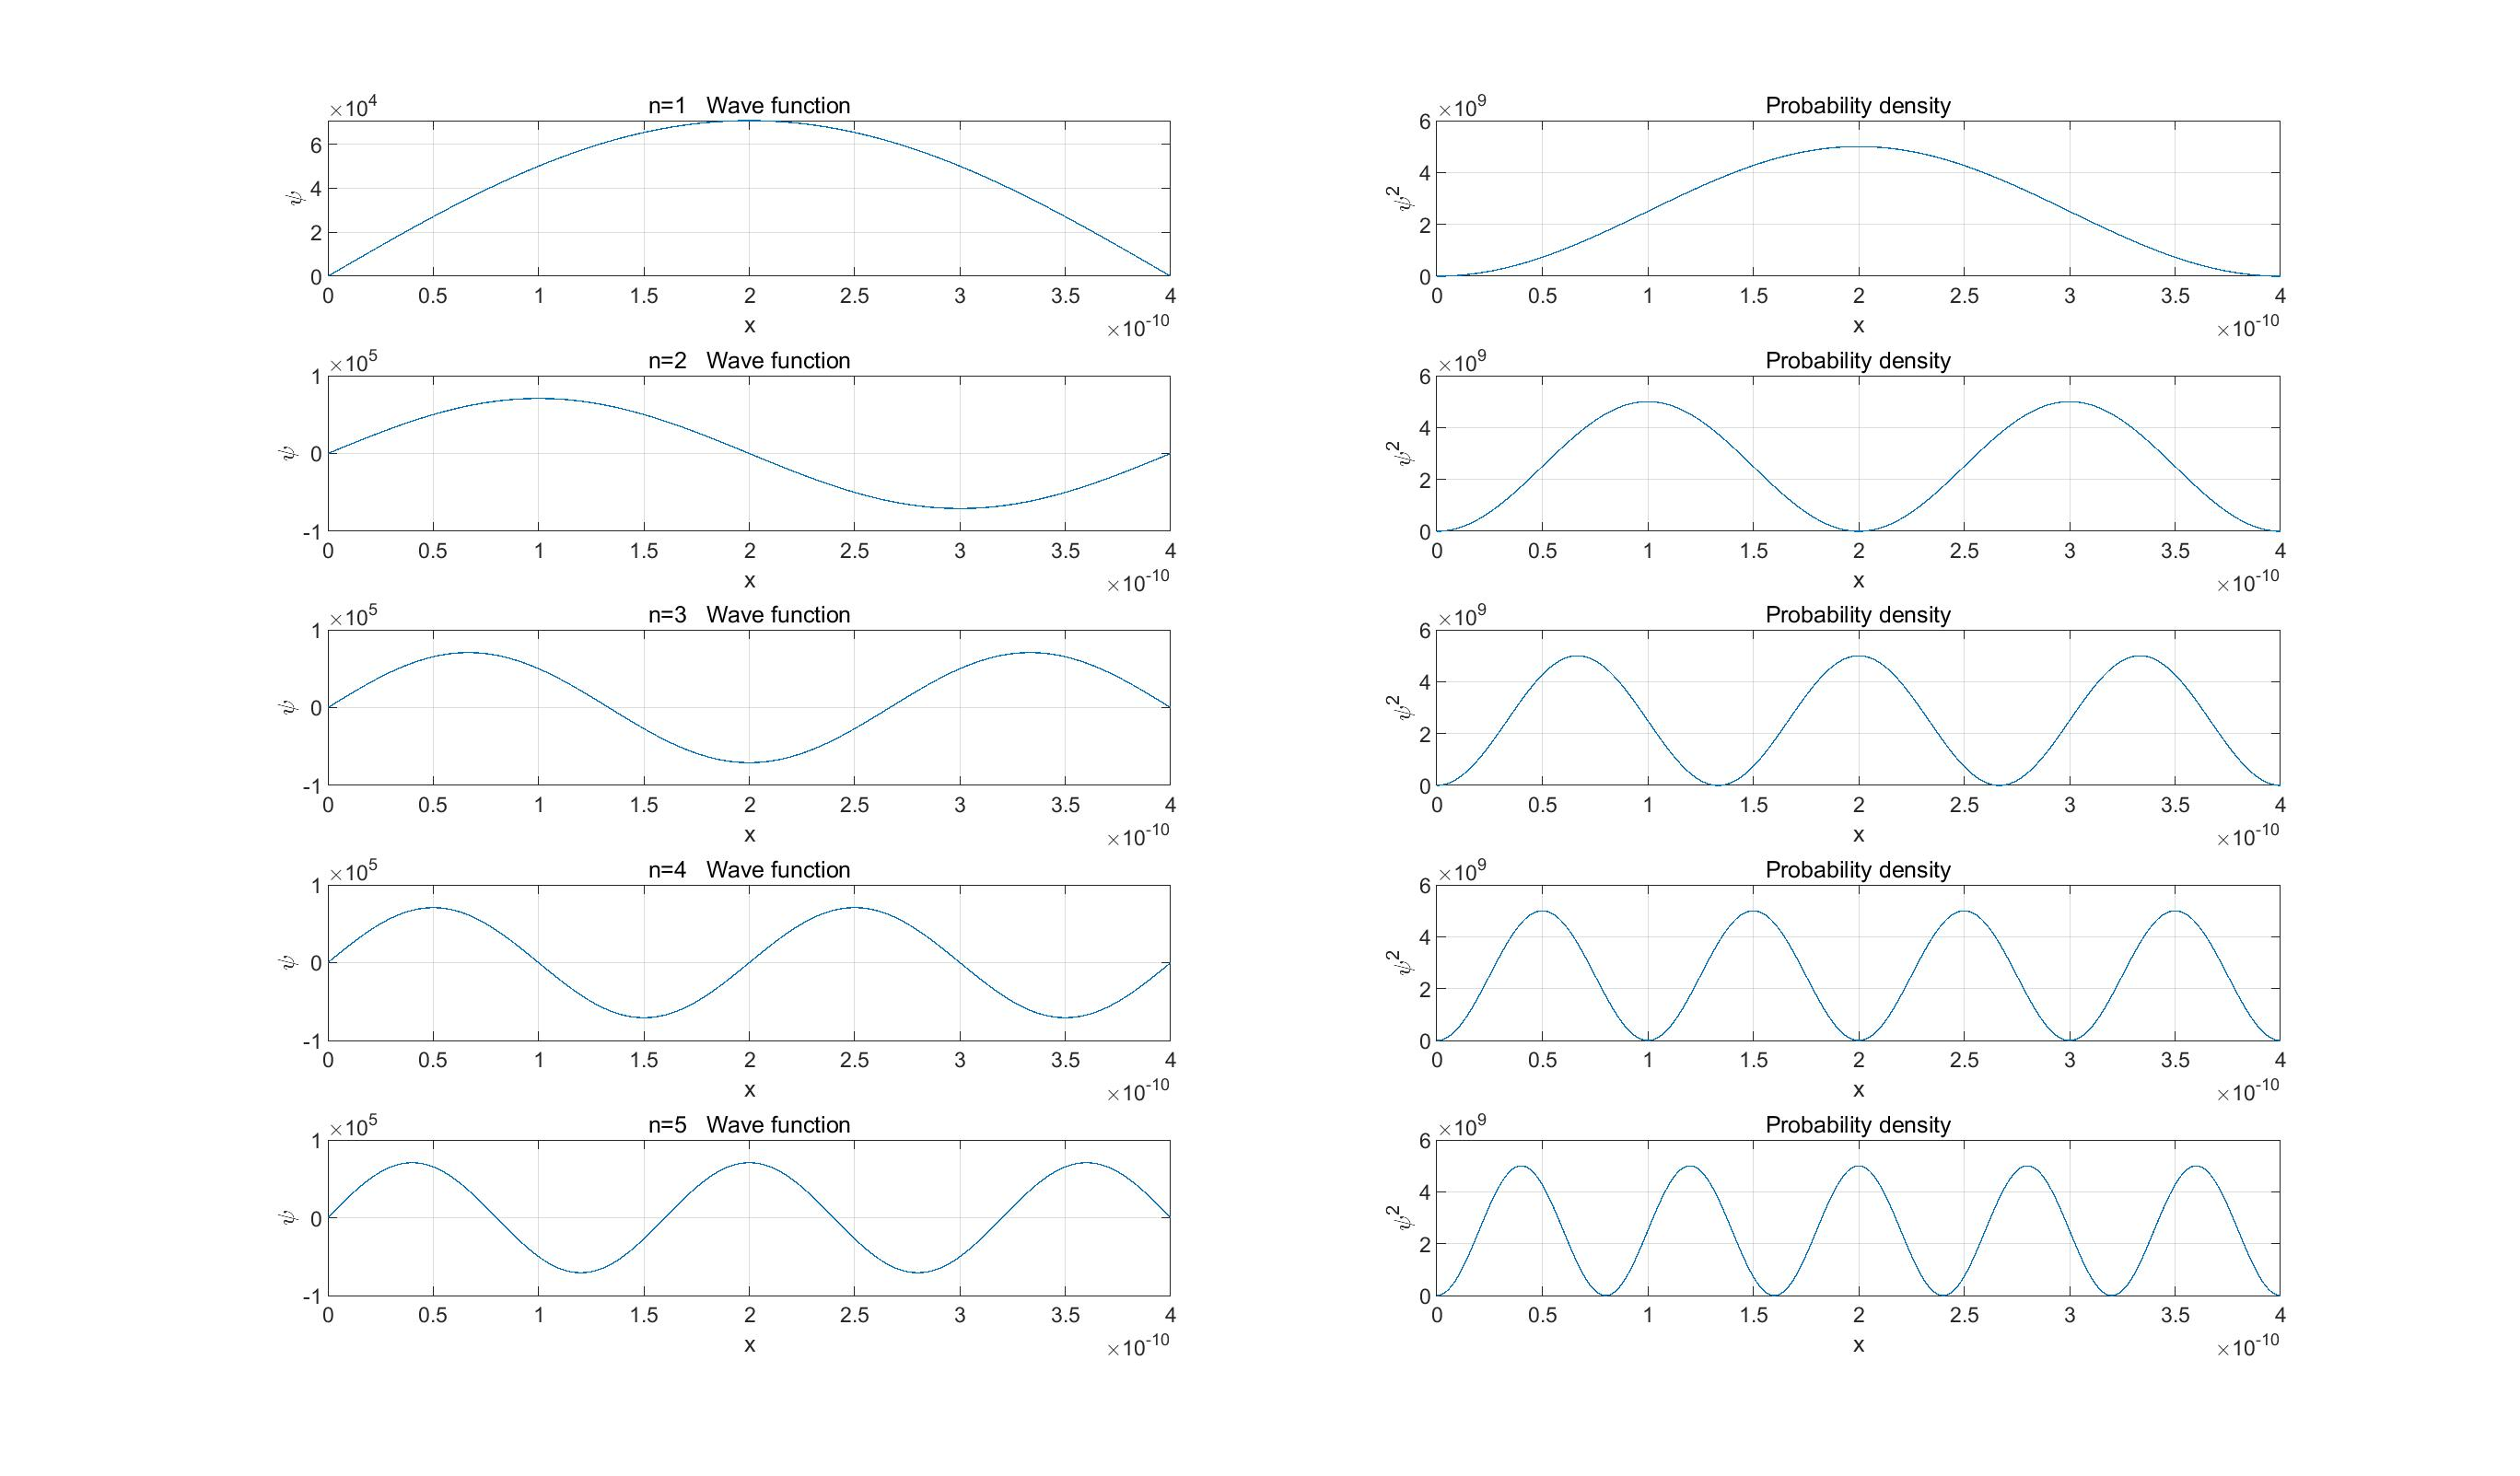
\includegraphics[width=0.9\textwidth]{figure/1Dinfinite.jpg}
    \caption{电子一维无限深势阱的波函数和概率密度示意图\footnote{其中$a=4\times 10^{-10}m$}}
    \label{infinite}
\end{figure}
\section{半无限深势阱}
本节我们讨论一个相对无限深势阱复杂的模型---半无限深势阱,其势能函数形式如下:
\begin{align}
V(x)=\left\{
    \begin{array}{ll}
       0  & 0\leq x\leq a \\
        +\infty & x<0\\
        V_0 & x>a
    \end{array}\right.
\end{align}

对于$0\leq x\leq a$的情况来说,方程形式与式\ref{equ3:string}完全一样,结合一边的边界条件,我们可以得到其通解同样为$\psi(x)=Bsinkx$,其中$k=\sqrt{\frac{2mE}{\hbar^2}}$。现在考虑$x>a$时的情况,事实上我们可以发现,方程同样可以写成式\ref{equ3:string}的形式:
\begin{equation}
    \frac{d^2\psi}{dx^2}+K^2\psi=0
\end{equation}

其中$K=\sqrt{\frac{2m(E-V)}{\hbar^2}}$。下面我们分别考虑几种可能的情况:
\begin{enumerate}
    \item $K<0$,此时$\psi(x)=CcosKx+DsinKx$,不满足波函数归一化推论:$\psi(+\infty)=0$的条件,固舍去;
    \item $K=0$,此时$\psi(x)=C+Dx$,同样不满足波函数归一化推论:$\psi(+\infty)=0$的条件,固舍去;
    \item $K>0$,此时$\psi(x)=Ce^{-Kx}+De^{Kx}$,由于波函数归一化推论:$\psi(+\infty)=0$,因此得到$D=0$,因此通解为$\psi(x)=Ce^{-Kx}$
\end{enumerate}

由于波函数应该是连续的,因此在$x=a$处的波函数与波函数的导数应该是对应相等的,即\footnote{这里波函数的导数相等是考虑到连续的定义,否则左右极限不相等,这个点无法用Schrodinger方程进行分析}:
\begin{align}
    \begin{split}\label{equ3:hinf_pre}
        Bsinka= & Ce^{-Kx}\\
        Bkcoska= & -CKe^{-Kx}
    \end{split}
\end{align}

两式相除,得到:
\begin{equation}\label{equ3:hinf}
    cotka=\frac{K}{k}
\end{equation}

这是一个超越方程,无法得到精确解,我们可以采用计算机数值求解的方法。在数学上,我们还可以通过将这个超越方程转化为两条函数曲线的交点问题,直观定性的对解进行分析。要想将问题转化为两条曲线的交点问题,需要统一等号两端的变量。令$X=ka,\beta=\sqrt{\frac{2mV_0}{\hbar^2}} a$,\footnote{我们常常称$\beta$ 为势场强度}于是式\ref{equ3:hinf}可以变为:
\begin{equation}
    cotX=-\sqrt{(\frac{\beta}{X})^2-1}
\end{equation}
%少图


通过图像,我们可以定性的得到一些结论:
\begin{enumerate}
    \item 由于$Y(\beta)=-\sqrt{(\frac{\beta}{X})^2-1}=0$,因此满足的能量本征态只有有限个;
    \item 与无限深势阱的驻波条件进行比较可以得,无限深势阱对应得$X=n\pi $,永远比半无限深势阱得$X$要大,并且两者之差越来越大。由图可知,当$n\rightarrow \infty $时,$n\pi-X_n\rightarrow \frac{\pi}{2}$。即两种模型的最大“能量”差;
    \item $X$的大小与取值与$\beta$息息相关。如果$\beta <\frac{\pi}{2}$,那么束缚态系统甚至没有符合条件的能量本征态
\end{enumerate}

通过图像,或是计算机得到$X_n$以后,就可以通过定义反解出能量本征值的值了:
\begin{equation}
    E_n=\frac{\hbar^2X^2}{2ma^2}
\end{equation}

同时根据归一化条件,我们可以得到一个含有系数$B_n,C_n$的方程:
\begin{equation}
    \int_0^a|\psi_n(x)|^2dx+\int_a^\infty|\varphi_n(x)|^2dx=1
\end{equation}

其中$\psi_n(x)=B_nsink_nx,\varphi_n(x)=C_ne^{-Kx}$。将上式与\ref{equ3:hinf_pre}中的任意一个方程联立即可得到展开系数$B_n,C_n$的值。

\section{对称与不对称的有限深势阱*}
有了半无限深势阱的求解方法,我们可以自然的迁移到两边的势能函数都是有限的情况。这个时候求解过程和半无限深势阱几乎一致,因此本节的结论请读者自行验证。
\section{直链共轭体系的$\pi$电子}
 本节我们讨论势阱问题的一个简单的例子。对于直链共轭体系的$\pi$电子来说,我们可以将其看作在$\sigma$键以及其它分子相互作用产生的势场里描述共轭体系的$\pi$电子的运动。当势场为周期函数等简单的函数时,其Schrodinger方程是可以精确求解的。我们考虑的模型时一个有$2N$个链状共轭体系的分子,其中N个碳碳单键,N个碳碳双键。此时我们令一根碳碳单键与一根碳碳双键组成的周期元素长度为l,假设其中2N个$\pi$电子在总长为$L=Nl$的无限深势阱内运动,那么可以知道,任意一个电子的能级都满足:
 \begin{equation}
     E_n=\frac{n^2h^2}{8mL^2}
 \end{equation}
 
 由于电子满足泡利不相容原理,因此同一个能级最多容纳自旋相反的两个电子,因此2N个$\pi$电子应该占据N个能级。那么当日光照射到这个有机物的时候,假如光子的频率正好满足:
 \begin{equation}
     hv_n=E_n-E_{n-1},n=2,3,\dots,N
 \end{equation}
 
 那么这个频率的光就会被吸收,我们联立电子的能级公式,可以得到:
 \begin{equation}
     v_n=\frac{h}{8mL^2}(2n-1),n=2,3,\dots,N
 \end{equation}
 
 得到了吸收的频率以后,我们可以求出吸收谱对应的波长:
 \begin{equation}
     \lambda_n=\frac{c}{v_n}=\frac{8mcl^2N^2}{h(2n-1)},n=2,3,\dots,N
 \end{equation}
 
 从上式中可以得出一些定性结论:
 \begin{enumerate}
     \item 当N固定,就会对应N-1个吸收峰,我们一般考察波长最长的那个峰,当日光照射到有机物的时候,波长小于该峰的光全部被吸收掉,如果此时剩下的光的波长落在了可见光区域,那么有机物就会呈现颜色。由该式我们可以明显看到,N越大,吸收带越宽,整个吸收谱会发生红移。
     \item 
 \end{enumerate}
\section{自由粒子的散射态问题}
    \subsection{方形势垒的隧穿效应}
    
    \subsection{势垒穿透的一种理解}
    对于势垒穿透问题,我们利用测不准原理给出一个解释:\footnote{注意,这里讲的只是一种理解而并不是严格解释}对于$E<V_0$的情况,当自由粒子进入$x=0$附近的区域,我们可以认为它的位置是比较精确的,由于测不准原理,其动量具有一定的取值范围,由于动量与能量之间存在关系:$E=\frac{p^2}{2m}$,所以能量就会具有一定的取值范围,此时就会出现能量大于势能$V_0$的情况。同理,我们考虑$E<V_0$的情况,此时根据上面的叙述,当粒子处于$x=0$附近时,由于位置可以比较精确的确定,此时能量具有一定的取值范围,就会有一些能量小于势能$V_0$被反射回去。
    \subsection{扫描隧道显微镜(STM)原理简介}
    扫描隧道显微镜是基于隧穿效应的的一种“电子显微镜”。它的具体原理是这样的(如图\ref{fig:STM}):简单说来就是利用一根探针(tip),在探针和样品的表面加上电压,如果探针和样品相距很近(大约是纳米级别的距离),由于电子的质量很小,根据,隧穿效应就会比较明显,探针上的原子就会穿过空隙(势垒)进入样品,形成极其微弱的电流。这样,我们通过记录电流的情况就能记录样品表面的精细结构。
    
    STM主要有两种工作模式:恒流模式(constant current mode)和恒高模式(constant height mode)\footnote{具体可以参考wiki的相关内容:$https://en.jinzhao.wiki/wiki/Scanning\_tunneling\_microscope$}。在恒流模式下,反馈电子调节高度通过一个电压到压电高度控制机构。如果在某一点的隧穿电流低于设定的水平(the set level),尖端就向样品移动,反之亦然。这种模式需要的时间较长,因为电子设备需要检查隧道电流,并在表面每个测量点的反馈回路中调整高度。当表面是原子级别的平面时,施加在z轴扫描器上的电压将主要反映局部电荷密度的变化。但当遇到原子台阶(atomic step),或当表面因重组而弯曲时,扫描器的高度也将因整体地形而改变。因此,当尖端扫描表面时,为了保持隧穿电流恒定,需要z轴扫描仪的电压形成的图像将包含地形和电子密度数据。在某些情况下,人们可能不清楚探针高度的变化是由其中的哪一种因素造成的。
    
    在恒定高度模式下,当扫描器在表面来回摆动时,z轴扫描器的电压保持恒定,并映射出与距离成指数关系的隧穿电流。这种操作方式更快,但在粗糙的表面上,可能存在大的吸附分子,可能会导致探针磨损。
    \begin{figure}[H]
        \centering
        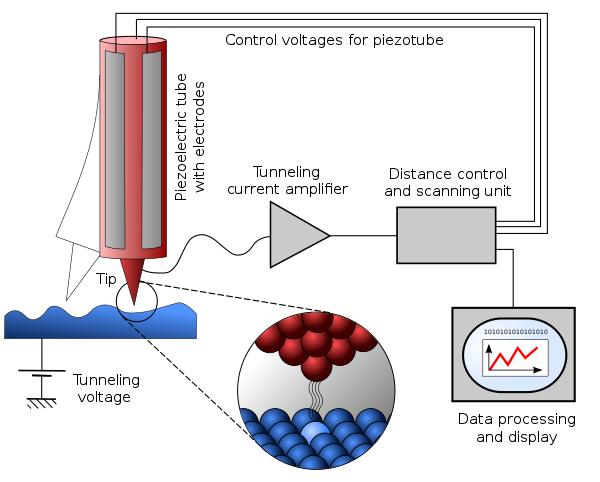
\includegraphics[width=0.9\textwidth]{figure/STM.png}
        \caption{扫描隧道显微镜的基本原理}
        \label{fig:STM}
    \end{figure}